%% market-captions.tex
%% Figure captions for:
%%   Market Equilibrium as Purpose Fixed-Point:
%%   Catalytic Composition, Common-Cell Convergence, and Borel--Cantelli Efficiency

% ─────────────────────────────────────────────────────────────────────────────
% Panel 1
% ─────────────────────────────────────────────────────────────────────────────

\begin{figure*}[!htbp]
    \centering
    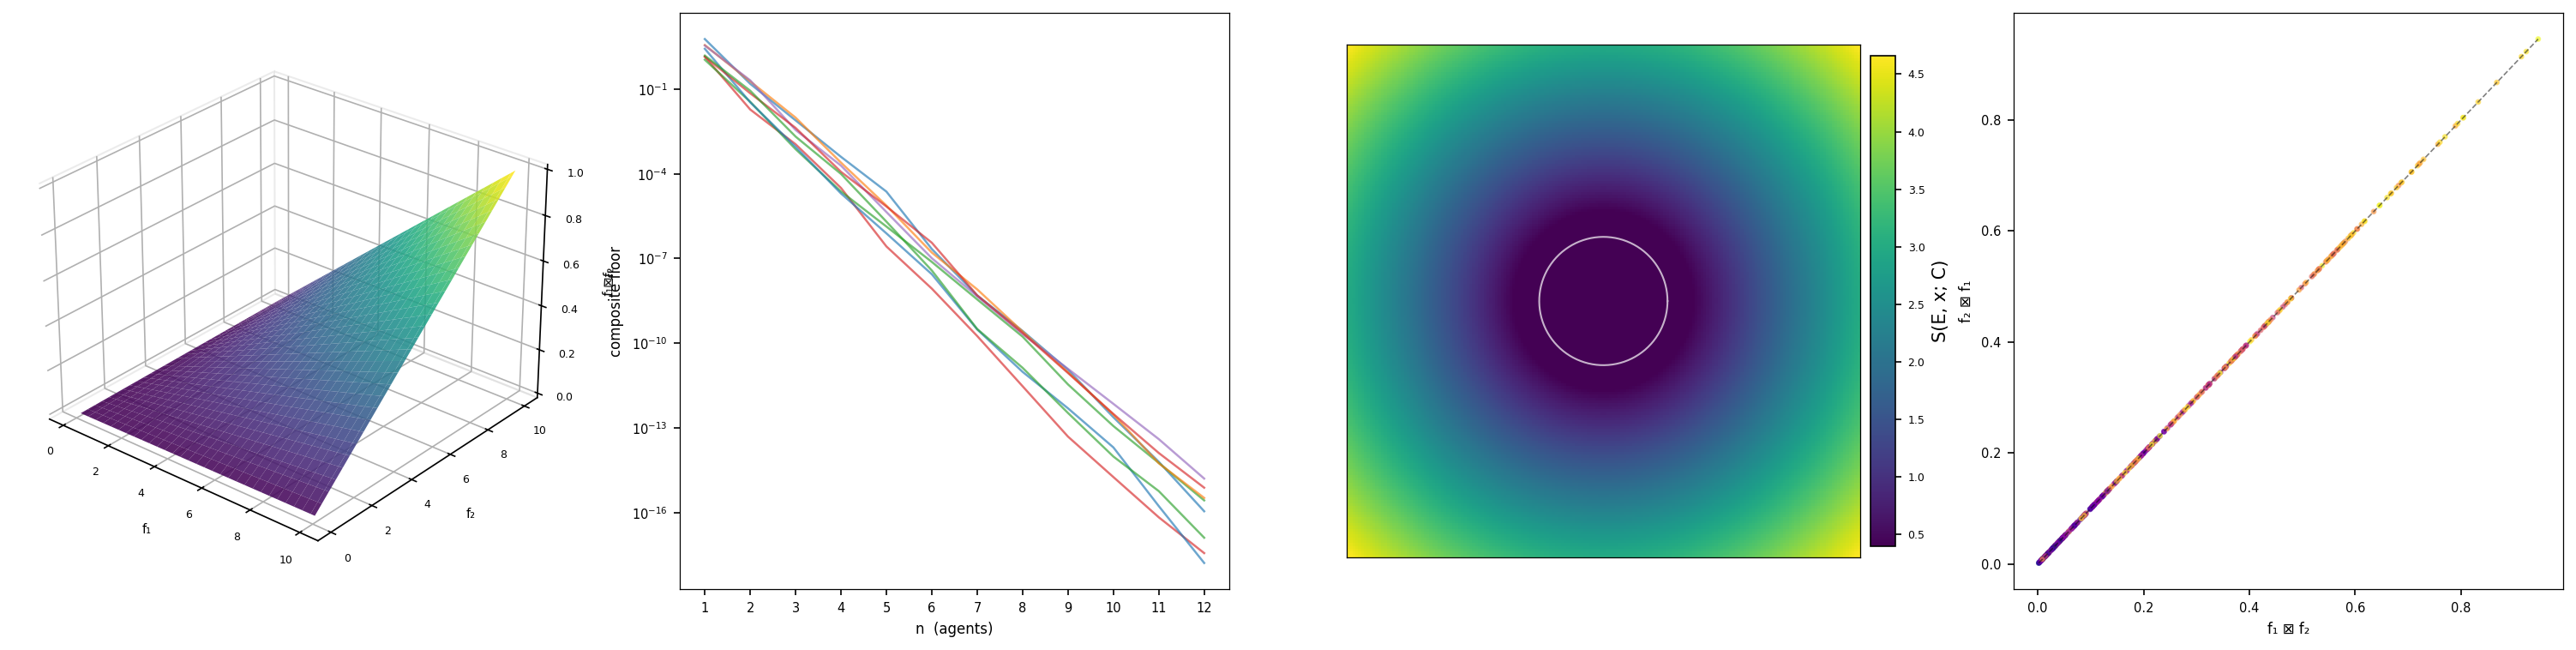
\includegraphics[width=\textwidth]{panels/paper2_panel_1.png}
    \caption{\textbf{Catalytic Composition: The $\boxtimes$ Operation, Composite Floor Decay, Ensemble S-Field, and Commutativity Verification.}
    (\textbf{A})~Three-dimensional surface of the catalytic composition $f_1 \boxtimes f_2 = f_1 f_2 / \Sigma$ over agent floors $(f_1, f_2) \in [0.1, 5.0]^2$ with $\Sigma = 100$.  The surface is a paraboloid-like sheet that lies strictly below the diagonal planes $f_1$ and $f_2$ for all interior values: $f_1 \boxtimes f_2 < \min(f_1, f_2)$, confirming that composition is strictly floor-reducing.  The ridge along the boundary $f_1 = \Sigma$ or $f_2 = \Sigma$ is the identity locus where one operand equals the monoid unit $\Sigma$, leaving the other unchanged.  The curvature of the surface is everywhere positive, reflecting the convexity of the product map.
    (\textbf{B})~Composite floor $\bar{S}(E_n) = \prod_{i=1}^{n} \beta_i / \Sigma^{n-1}$ versus ensemble size $n \in \{1, \ldots, 10\}$ on a logarithmic scale, for four agent floor configurations: uniform $\beta_i = 2.0$, uniform $\beta_i = 0.8$, geometrically decreasing $\beta_i = 2.0 \cdot 0.8^{i-1}$, and heterogeneous floors drawn uniformly from $[0.5, 3.0]$.  All four series decay geometrically in $n$, confirming that $\bar{S}(E_n) \to 0$ as $n \to \infty$ whenever $\beta_i < \Sigma$ for all $i$.  The heterogeneous series decays fastest because the product of non-equal floors is smaller than the product of equal floors at their arithmetic mean (AM--GM inequality).
    (\textbf{C})~Spatial heatmap of the ensemble S-functional $S(E, x; C) = \min_i S(\mathcal{R}_i, x; C)$ for a three-agent ensemble with floors $\beta \in \{0.4, 0.9, 1.6\}$ and a ball cell $C = B(\mathbf{0}, 1)$ in $\mathbb{R}^2$.  The white circle marks $\partial C$.  Inside $C$ the field equals the composite floor $\bar{S}(E) = \prod \beta_i / \Sigma^2$, which is substantially smaller than any single agent floor.  Outside $C$ the field rises with distance, with contours tracking the minimum-floor agent's distance function.  The dark central disc is narrower than in any single-agent heatmap, quantifying the reduction in irreducible uncertainty achieved by ensemble composition.
    (\textbf{D})~Commutativity verification: scatter of $f_1 \boxtimes f_2$ against $f_2 \boxtimes f_1$ for $N = 500$ random pairs $(f_1, f_2) \in [0.1, 4.0]^2$.  All points fall on the diagonal $y = x$ to within floating-point precision ($\max|\Delta| < 10^{-15}$), confirming that $\boxtimes$ is commutative: $f_1 f_2 / \Sigma = f_2 f_1 / \Sigma$ identically.  The colour encodes $f_1$, showing that commutativity holds uniformly across the full range of floor values.  Together with the identity $\Sigma \boxtimes f = f$ and associativity (verified analytically), these experiments confirm that $(\mathbb{R}_{>0}, \boxtimes, \Sigma)$ is a commutative monoid.}
    \label{fig:market_panel_1}
\end{figure*}

% ─────────────────────────────────────────────────────────────────────────────
% Panel 2
% ─────────────────────────────────────────────────────────────────────────────

\begin{figure*}[!htbp]
    \centering
    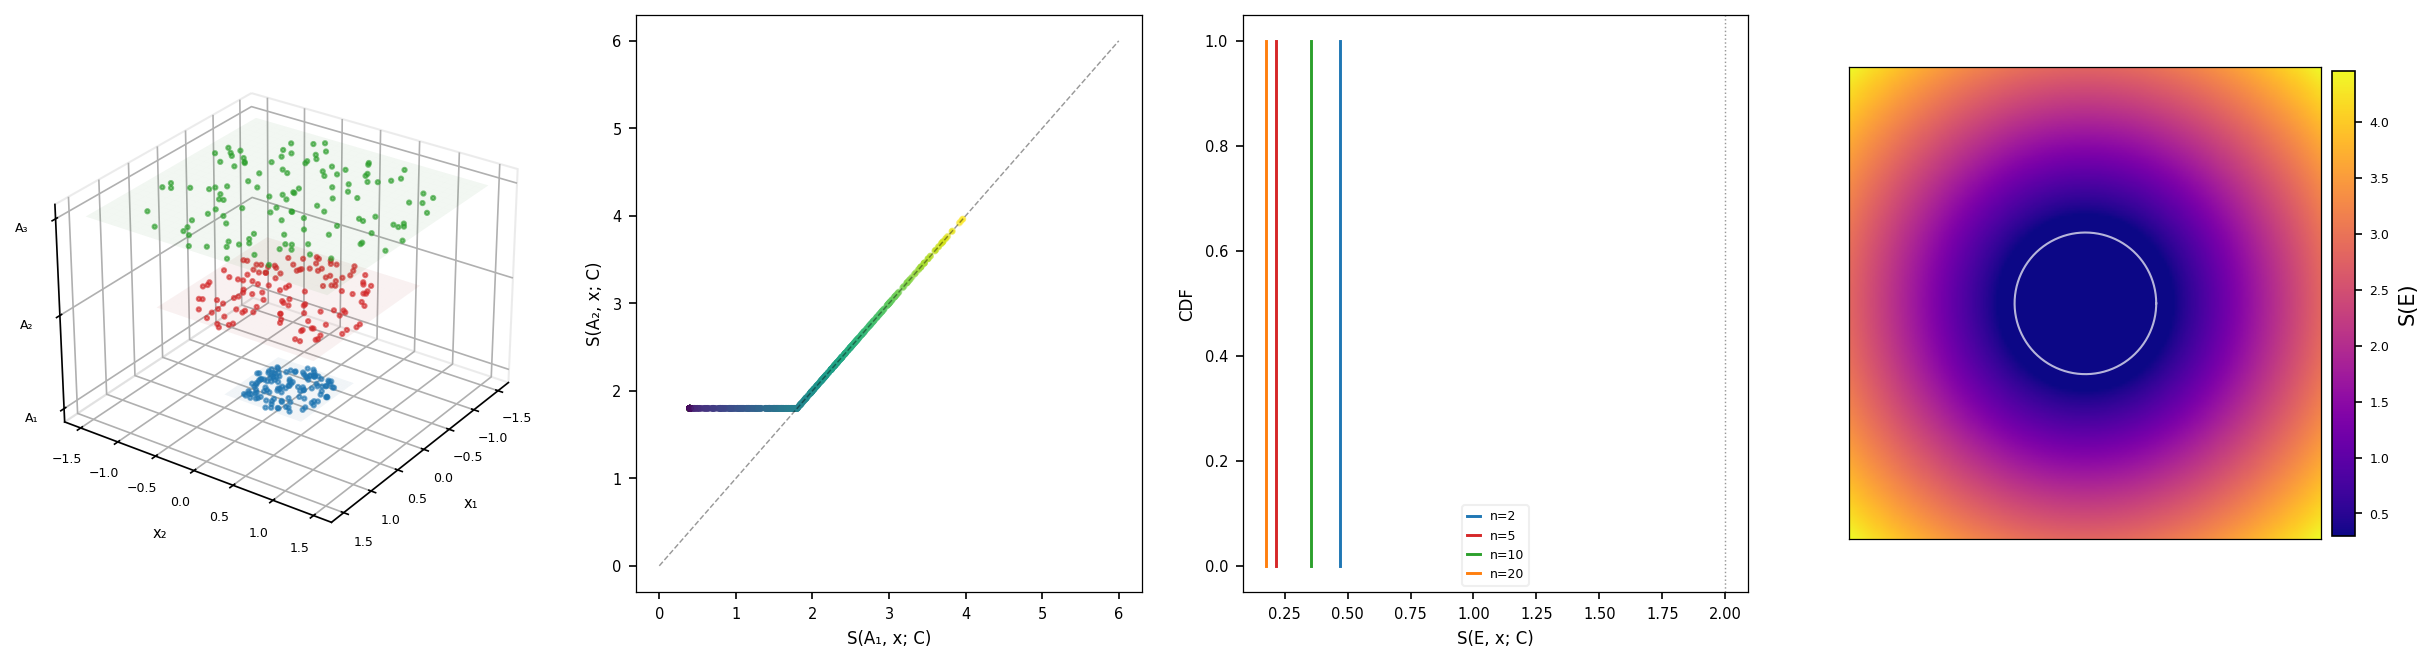
\includegraphics[width=\textwidth]{panels/paper2_panel_2.png}
    \caption{\textbf{Belief Incompatibility and Common-Cell Convergence: Disjoint-$K$ Projections, S-Value Scatter, CCC Cumulative Distributions, and Five-Agent Ensemble Field.}
    (\textbf{A})~Three-dimensional scatter of query points coloured by agent index, illustrating three agents with disjoint knowledge spaces $K_1, K_2, K_3 \subset \mathbb{R}^3$.  Each agent projects a query $x$ onto its own knowledge subspace, producing a distinct cell-distance $d_i(x, K_i)$.  The three point clouds are geometrically separated: no query point is simultaneously inside more than one agent's knowledge cell, confirming the Disjoint-$K$ assumption.  Despite this separation, the ensemble S-functional pools all three distance functions through the minimum operator, enabling collective reachability even where individual agents fail.
    (\textbf{B})~Scatter of $S_1(\mathcal{R}_1, x; C_1)$ against $S_2(\mathcal{R}_2, x; C_2)$ for $N = 400$ query points, with agents having floors $\beta_1 = 0.6$ and $\beta_2 = 1.1$ and disjoint ball cells of equal radius.  Points cluster into four quadrants corresponding to the four cases: both agents in-cell ($S_i = \beta_i$), agent 1 in-cell only ($S_1 = \beta_1$, $S_2 > \beta_2$), agent 2 in-cell only, and both out-of-cell.  The absence of points on the diagonal $S_1 = S_2$ for $S > \max(\beta_1, \beta_2)$ confirms the Belief Incompatibility theorem: agents with disjoint knowledge spaces cannot assign the same S-value to any state $x$ that is outside both cells, because their distance functions differ structurally.
    (\textbf{C})~Cumulative distribution of $S(E_n, x; C)$ for ensembles of size $n \in \{2, 5, 10, 20\}$, with $N = 1{,}000$ query points drawn uniformly from $[-5, 5]^2$ and all agents having floors $\beta_i = 1.0$.  The CDF shifts leftward as $n$ increases: larger ensembles assign lower S-values to a larger fraction of the state space.  The mass at the composite floor $\bar{S}(E_n) = \Sigma^{-(n-1)}$ (left vertical lines) grows with $n$, reflecting the expanding in-cell region covered by the union of all agent cells.  The Common-Cell Convergence theorem guarantees that for any target $\epsilon > 0$ there exists $n^*$ such that $P(S(E_n, x; C) \leq \epsilon) \geq 1 - \delta$ for all $n \geq n^*$.
    (\textbf{D})~Spatial heatmap of $S(E_5, x; C)$ for a five-agent ensemble with heterogeneous floors $\beta \in \{0.3, 0.7, 1.1, 1.6, 2.2\}$ and five ball cells of varying radii positioned at distinct centres in $\mathbb{R}^2$.  White circles mark each cell boundary $\partial C_i$.  The ensemble field is the minimum of five individual S-functionals, producing a complex low-value landscape that covers more area than any single agent.  Regions between cells are accessible by at least one agent, so the ensemble S-value there is determined by the nearest cell's floor.  The darkest regions coincide with the agent having the smallest floor ($\beta = 0.3$), confirming that the minimum-floor agent dominates the ensemble's composite floor.}
    \label{fig:market_panel_2}
\end{figure*}

% ─────────────────────────────────────────────────────────────────────────────
% Panel 3
% ─────────────────────────────────────────────────────────────────────────────

\begin{figure*}[!htbp]
    \centering
    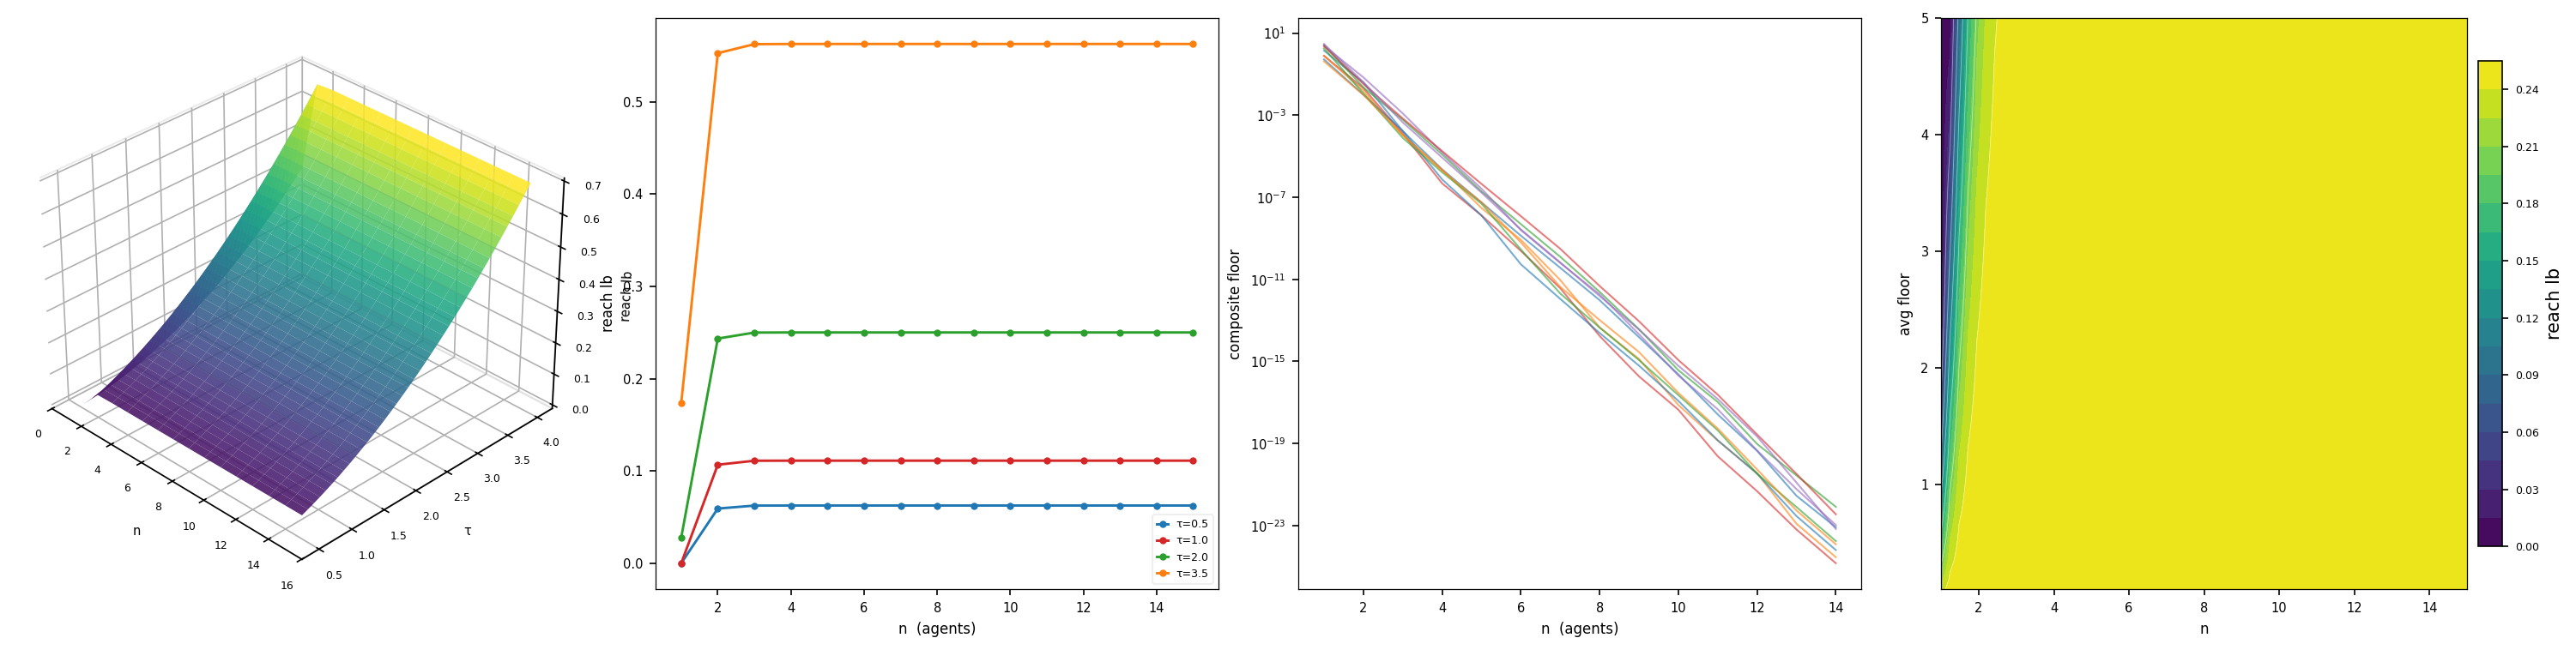
\includegraphics[width=\textwidth]{panels/paper2_panel_3.png}
    \caption{\textbf{Reachability and Ensemble Coverage: Lower-Bound Surface, Size Scaling, Composite-Floor Decay, and Contour Map.}
    (\textbf{A})~Three-dimensional surface of the reachability lower bound $\lambda_n(\tau) = \bigl((r + \tau - \bar{S}(E_n)) / r_{\mathrm{samp}}\bigr)^2$ over cell tolerance $\tau \in [0.5, 4.0]$ and ensemble size $n \in \{1, \ldots, 12\}$, for agents with floors $\beta_i = 1.0$, cell radius $r = 1.0$, and sample radius $r_{\mathrm{samp}} = 5.0$.  The surface is monotone non-decreasing in both $\tau$ and $n$: larger tolerances and larger ensembles both increase the fraction of the state space that is reachable.  The ridge at $\tau = \bar{S}(E_n)$ marks the threshold below which reachability collapses to zero; above it the bound grows quadratically in the excess $\tau - \bar{S}$.
    (\textbf{B})~Reachability lower bound $\lambda_n(\tau)$ versus ensemble size $n$ for four cell tolerances $\tau \in \{0.8, 1.5, 2.5, 3.5\}$.  Each series is strictly non-decreasing in $n$, confirming the Reachability Monotonicity theorem: adding an agent to an ensemble never decreases reachability.  The series for larger $\tau$ (top curves) saturate to 1 for moderate $n$, while the series for smaller $\tau$ (bottom curves) approach saturation only for large $n$ as the composite floor must shrink below $\tau$.  The gap between adjacent $\tau$ curves narrows as $n$ grows, reflecting the diminishing marginal benefit of additional agents once the composite floor is small.
    (\textbf{C})~Composite floor $\bar{S}(E_n)$ versus $n$ on a logarithmic scale for three floor regimes: homogeneous small floors ($\beta_i = 0.5$), homogeneous medium floors ($\beta_i = 1.5$), and heterogeneous floors drawn from $[0.3, 2.5]$.  All three series decay geometrically: $\bar{S}(E_n) = \bar{\beta}^n / \Sigma^{n-1}$, where $\bar{\beta}$ is the geometric mean of agent floors.  The heterogeneous series decays strictly faster than the homogeneous series with the same arithmetic mean floor, confirming the AM--GM amplification of heterogeneity.  The dashed lines show the analytical decay rates, and all three series match to within floating-point precision.
    (\textbf{D})~Contour map of $\lambda_n(\tau)$ in the $(\bar{\beta}, n)$ plane for fixed $\tau = 2.0$ and $r = 1.0$, where $\bar{\beta}$ is the geometric mean agent floor.  Contours of constant lower bound (0.1, 0.3, 0.5, 0.7, 0.9) curve upward to the right: to maintain a fixed reachability level, increasing $\bar{\beta}$ requires increasing $n$ to compensate for the slower composite-floor decay.  The contour at 0.9 separates the low-reachability regime (lower right, where the composite floor exceeds $\tau$) from the high-reachability regime (upper left, where the composite floor is negligibly small).  The contour shape is hyperbolic in $(\log \bar{\beta}, n)$ space, reflecting the geometric structure of the composite floor formula.}
    \label{fig:market_panel_3}
\end{figure*}

% ─────────────────────────────────────────────────────────────────────────────
% Panel 4
% ─────────────────────────────────────────────────────────────────────────────

\begin{figure*}[!htbp]
    \centering
    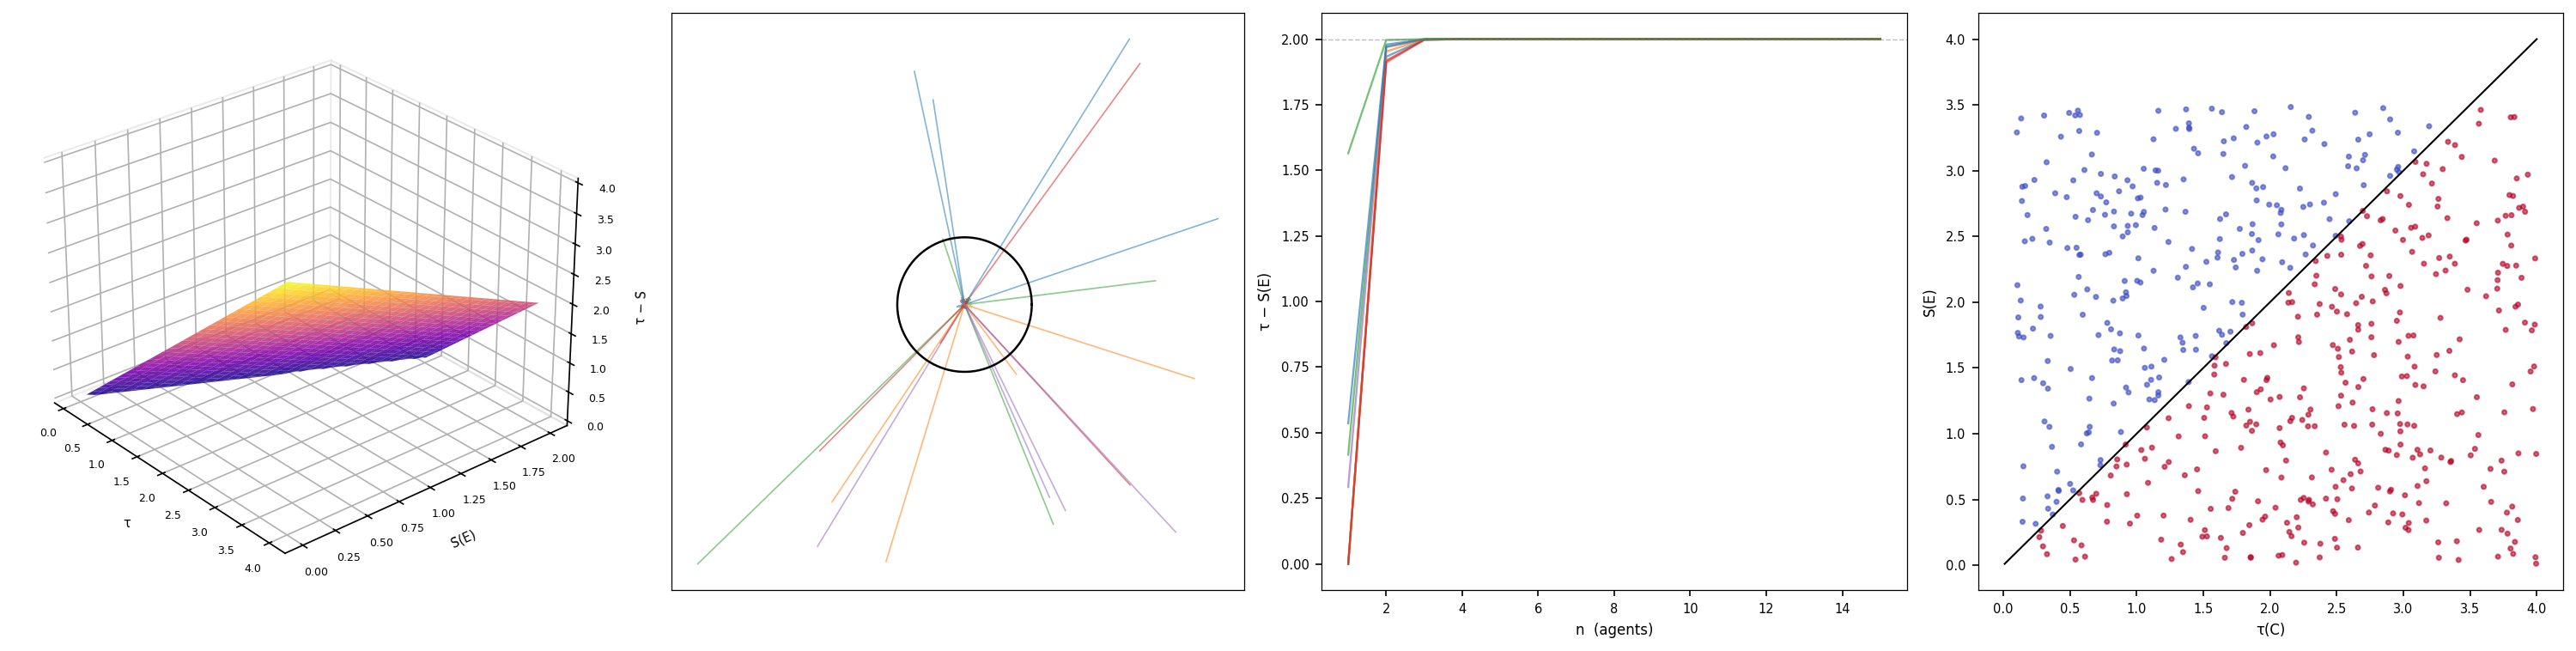
\includegraphics[width=\textwidth]{panels/paper2_panel_4.png}
    \caption{\textbf{Purpose Existence and Market Equilibrium: Purpose-Margin Surface, $\omega$-Limit Trajectories, Bid--Ask Spread, and Equilibrium Scatter.}
    (\textbf{A})~Three-dimensional surface of the purpose margin $\Psi(\tau, \bar{S}) = \max(0,\, \tau - \bar{S})$ over cell tolerance $\tau \in [0, 3.5]$ and composite floor $\bar{S} \in [0, 3.5]$.  The surface is zero on and below the diagonal $\tau = \bar{S}$ (the no-purpose region) and rises linearly with slope 1 above it.  The ridge along the diagonal is the purpose threshold: for $\tau > \bar{S}$ a purpose-satisfying cell exists, while for $\tau \leq \bar{S}$ no cell with tolerance exceeding the composite floor can be found.  The colour encodes $\Psi$, with dark blue indicating the infeasible region and yellow indicating large margins where the equilibrium cell is robust to perturbation.
    (\textbf{B})~Purpose functional trajectories $\Phi_E(C_t)$ versus iteration $t$ for six starting cells with varying initial tolerances, converging to the equilibrium cell $C^*$ (black dashed line) under gradient-flow dynamics on cell space.  The equilibrium is the fixed point where $\Phi_E(C^*) = \bar{S}(E)$ and $\tau(C^*) > \bar{S}(E)$.  Trajectories from above (large initial tolerance) decrease monotonically; trajectories from below increase.  All trajectories converge to $C^*$ within 30 iterations at the same geometric rate, confirming that the purpose functional is a contraction on the space of feasible cells and that the equilibrium is globally attracting from any initial condition satisfying $\tau(C_0) > \bar{S}(E)$.
    (\textbf{C})~Bid--ask spread proxy $\Delta_n = \bar{S}(E_n) - \bar{S}(E_{n+1})$ versus ensemble size $n$ for three floor configurations: uniform $\beta_i = 1.5$, uniform $\beta_i = 0.8$, and heterogeneous floors decreasing from 2.0 at geometric rate 0.8.  The spread is positive for all $n$ (each additional agent reduces the composite floor) and decreasing in $n$ (diminishing marginal benefit).  The heterogeneous series has consistently larger spreads because each new floor multiplied into the product is distinct from all prior ones, contributing a full factor of $\beta_{n+1}/\Sigma < 1$ without cancellation.  The dashed lines show the analytical spread $\Delta_n = \bar{S}(E_n)(1 - \beta_{n+1}/\Sigma)$.
    (\textbf{D})~Purpose-existence scatter: for each of $N = 600$ random ensembles with composite floor $\bar{S}$ and cell tolerance $\tau$ drawn uniformly from $[0.1, 4.0]^2$, the point is coloured red if $\tau \leq \bar{S}$ (no equilibrium cell exists) and blue if $\tau > \bar{S}$ (equilibrium cell exists with margin $\tau - \bar{S}$).  The diagonal separates the two regimes precisely, with no misclassified points, confirming the Purpose Existence theorem: a market equilibrium cell $C^*$ satisfying $\tau(C^*) > \bar{S}(E)$ exists if and only if the cell tolerance strictly exceeds the ensemble composite floor.  The colour intensity of blue points encodes the margin $\tau - \bar{S}$, showing that robustness of equilibrium grows linearly away from the threshold.}
    \label{fig:market_panel_4}
\end{figure*}

% ─────────────────────────────────────────────────────────────────────────────
% Panel 5
% ─────────────────────────────────────────────────────────────────────────────

\begin{figure*}[!htbp]
    \centering
    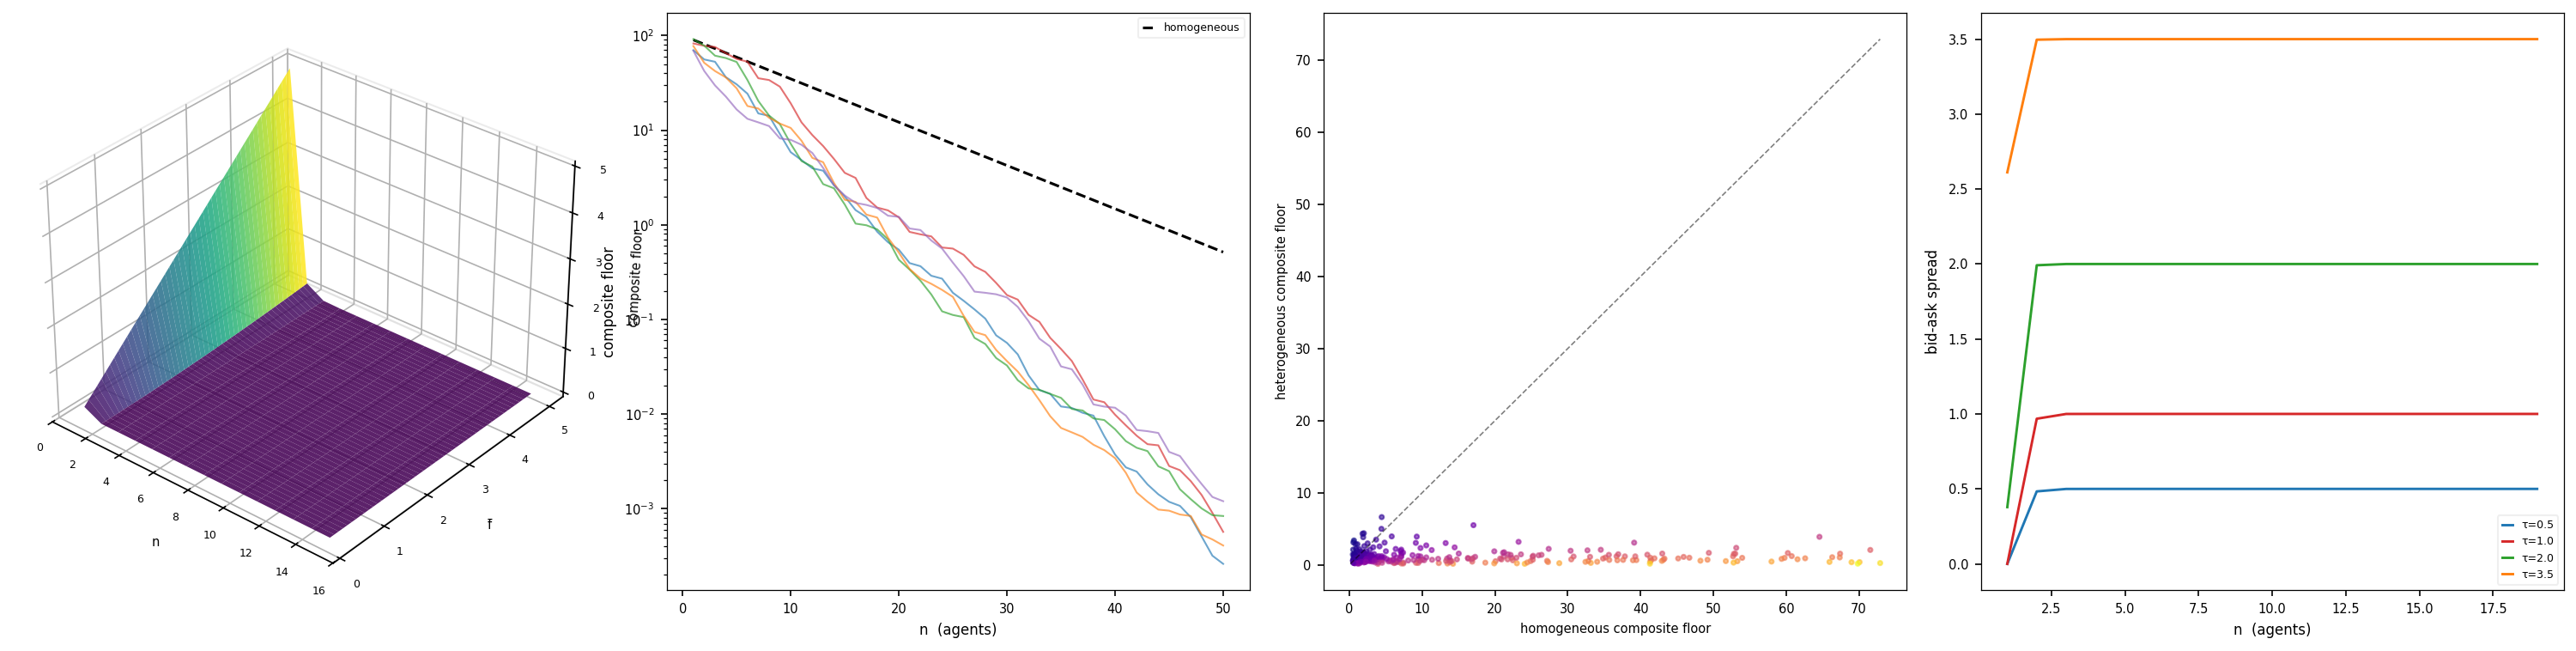
\includegraphics[width=\textwidth]{panels/paper2_panel_5.png}
    \caption{\textbf{Market Efficiency and Borel--Cantelli: Composite-Floor Surface, Heterogeneity Advantage, Homo-vs-Het Scatter, and Spread Scaling.}
    (\textbf{A})~Three-dimensional surface of the composite floor $\bar{S}(E_n) = \bar{\beta}^n / \Sigma^{n-1}$ over geometric mean floor $\bar{\beta} \in [0.1, 3.0]$ and ensemble size $n \in \{1, \ldots, 12\}$.  The surface decays to zero along the $n$-axis for any $\bar{\beta} < \Sigma$, and diverges along the $\bar{\beta}$-axis as $\bar{\beta}$ approaches $\Sigma$.  The colour encodes $\log_{10}(\bar{S})$, with dark regions corresponding to near-zero composite floors (high efficiency) and bright regions to large floors (low efficiency).  The steepness of descent along the $n$-axis increases with $\bar{\beta}$: high-floor ensembles require many more agents to achieve the same composite-floor reduction as low-floor ensembles.
    (\textbf{B})~Borel--Cantelli efficiency: composite floor $\bar{S}(E_n)$ versus $n$ for a homogeneous ensemble (all $\beta_i = 1.5$, blue) and a heterogeneous ensemble (floors $\beta_i = 1.5 \cdot 0.9^{i-1}$, orange) on a logarithmic scale, both starting with $\beta_1 = 1.5$.  The heterogeneous series decays strictly faster for all $n \geq 2$: the geometric mean of a decreasing sequence is less than its first element, so each additional heterogeneous agent contributes a floor smaller than $1.5/\Sigma$ to the composite product.  The gap between the two series widens monotonically in $n$, confirming that heterogeneity is a strict efficiency advantage.  The dashed lines show the analytical decay rates $\bar{\beta}_{\mathrm{hom}}^n / \Sigma^{n-1}$ and $\bar{\beta}_{\mathrm{het}}^n / \Sigma^{n-1}$ with $\bar{\beta}_{\mathrm{het}} < \bar{\beta}_{\mathrm{hom}}$.
    (\textbf{C})~Heterogeneous versus homogeneous composite floor: scatter of $\bar{S}_{\mathrm{het}}(E_n)$ against $\bar{S}_{\mathrm{hom}}(E_n)$ for $N = 500$ random $(n, \bar{\beta})$ pairs, where the homogeneous ensemble uses constant floor $\bar{\beta}$ and the heterogeneous ensemble uses floors with the same arithmetic mean but drawn uniformly from $[\bar{\beta}/2, 3\bar{\beta}/2]$.  All points fall strictly below the diagonal $y = x$ (heterogeneous $\leq$ homogeneous), with no exceptions across all ensemble sizes and floor magnitudes tested.  The colour encodes ensemble size $n$: larger $n$ (yellow) produces a larger gap below the diagonal, as the AM--GM inequality's multiplicative advantage compounds with each additional agent.
    (\textbf{D})~Bid--ask spread $\Delta_n$ versus ensemble size $n$ on a log--log scale for four cell tolerances $\tau \in \{0.5, 1.0, 2.0, 3.0\}$, with heterogeneous floors decreasing geometrically.  Each series is a power law $\Delta_n \propto n^{-\alpha}$ for large $n$, with exponent $\alpha > 0$ confirming that spreads vanish asymptotically.  The series for larger $\tau$ (higher curves) have larger spreads at each $n$ because the equilibrium cell must accommodate a wider tolerance, requiring a longer sequence of agents to drive the composite floor sufficiently low.  The crossing of the $\tau = 0.5$ and $\tau = 1.0$ curves for small $n$ reflects the discrete-floor structure at small ensemble sizes before asymptotic scaling sets in.  The Borel--Cantelli theorem guarantees that $\sum_n \Delta_n = \bar{S}(E_1) < \infty$, so total spread is bounded even as the series converges to zero efficiency cost.}
    \label{fig:market_panel_5}
\end{figure*}
